\documentclass[12pt,a4paper]{article}
\usepackage[utf8]{inputenc}
\usepackage{graphicx}
\usepackage{color}
\usepackage[magyar]{babel}
\usepackage{listings}
\usepackage{float}

\usepackage{enumerate}
\usepackage{tikz}
\usetikzlibrary{shapes,arrows}
\usetikzlibrary{positioning}
\usetikzlibrary{arrows.meta}

\tikzset{
block/.style = {draw, fill=white, rectangle, minimum height=3em, minimum width=3em},
tmp/.style  = {coordinate}, 
input/.style = {coordinate},
output/.style= {coordinate},
pinstyle/.style = {pin edge={to-,thin,black}
}
}
\usepackage[siunitx]{circuitikz} 
\renewcommand{\lstlistingname}{Lista}
\usepackage{hyperref}
\hypersetup{
	pdftitle={HA5KFU tanfolyam - Modulációs gyakorlat},
	pdfauthor={HA5KFU Rádióamatőr Klub},
	pdfsubject={HA5KFU tanfolyam},
	pdfcreator={latex},
	pdfkeywords={ },
	pdfpagemode=UseOutlines,
	pdfdisplaydoctitle=true,
	pdflang=hu,
	unicode
}
\usepackage{color} %red, green, blue, yellow, cyan, magenta, black, white
\definecolor{mygreen}{RGB}{28,172,0} % color values Red, Green, Blue
\definecolor{mylilas}{RGB}{170,55,241}
\lstset{language=Matlab,%
	basicstyle=\scriptsize\ttfamily,
    %basicstyle=\color{red},
    breaklines=true,%
    morekeywords={matlab2tikz},
    keywordstyle=\color{blue},%
    morekeywords=[2]{1}, keywordstyle=[2]{\color{black}},
    identifierstyle=\color{black},%
    stringstyle=\color{mylilas},
    commentstyle=\color{mygreen},%
    showstringspaces=false,%without this there will be a symbol in the places where there is a space
    numbers=left,%
    numberstyle={\tiny \color{black}},% size of the numbers
    numbersep=9pt, % this defines how far the numbers are from the text
    emph=[1]{for,end,break},emphstyle=[1]\color{red}, %some words to emphasise
    %emph=[2]{word1,word2}, emphstyle=[2]{style},    
}

\pagestyle{plain}
\sloppy
\begin{document}
\begin{center}

\includegraphics[width=300pt,keepaspectratio]{figures/ha5kfu.eps}
\\[0.5cm]
Rádióamatőr tanfolyamot segítő jegyzet, egyelőre kidolgozás alatt \\
Összeállította: Szabó Áron % Feel free to add yourself
\\[1cm]

{\huge \bfseries Modulációs gyakorlat \\[2cm]}



\end{center}

\renewcommand{\contentsname}{Tartalom}\tableofcontents 
\newpage

\newpage

\section{Bevezető}
A workshop célja bemutatni a különböző modulációs eljárások idő- és frekvenciatartománybeli viselkedését, illetve matematikai leírásukat. 

\section{Előkészületek}
A workshop Octave-ban és Matlab-ban is elvégezhető, a használt parancsok mindkettőben működőképesek.

\paragraph{Octave telepítés:} 
\begin{itemize}
	\item \textbf{GNU Octave telepítése:} \\\url{https://wiki.octave.org/Category:Installation}
	\item \textbf{Signal package telepítése:} Octave-on belül: 	\\
	\texttt{pkg install -forge signal}\\
	Ha ez valamiért nem működne, akkor Ubuntun command line-ból is telepítheted: \texttt{sudo apt-get install octave-signal}
\end{itemize}

\section{Feladatok}

\subsection{Szinusz jel generálása, ábrázolása}
Első feladatunk egy szinusz jel generálása lesz, melyet a \textit{sin()} függvénnyel tehetünk meg. Fontos, hogy ez a függvény egy adott érték szinuszát adja vissza, nekünk viszont egy időtartománybeli függvényre van szükségünk. 

Létre kell hoznunk tehát egy időtengelyt, aminek pontjaiban kiszámoljuk a függény értékét. Ebből a szempontból fontos meghatározni a mintavételi frekvenciát ($F_s$), hiszen ebből az értékből számolható, hogy két minta közt mennyi idő fog eltelni. Válasszuk a mintavételi frekvenciát \textit{44 100 Hz}-re, ami a digitális audió jelfeldolgozásban használatos frekvencia, és a számítógép hangkártyáján könnyen lejátszható.

Ha a minták számát ($N$) másodpercben szeretnénk megadni, egyszerűen szorozzuk meg a másodperc értéket a mintavételi frekvenciával. A másodperc időtengelyt ($t$) úgy kaphatjuk meg, ha az \texttt{1:N} sorozatot elemenként elosztjuk a mintavételi frekvenciával (a transzponálásra azért van szükség, hogy oszlopvektort kapjunk). Ez után a szinusz jel egyszerűen kiszámolható: mivel a szinusz egy periódusa $2\pi$, a szinuszjel pillanatnyi értékét $t \cdot f \cdot 2\pi$-re kell választani, ahol $f$ a szinusz frekvenciája.

\begin{lstlisting}[frame=single,language=matlab,caption=Mintavételi frekvencia beállítása és szinuszjel előállítása]
Fs = 44100; % mintaveteli freki
l = 1.5; % minta hossza masodpercben
N = l * Fs, % mintak szama
f = 440; % 20 Hz-es lesz a jel
t = ( 1:N )' ./ Fs; % Ido oszlopvektora
y = sin( t * f * 2 * pi );
plot( t, y );
\end{lstlisting}

Ábrázoljuk a Plot függvénnyel időtartományban:

\begin{figure}[H]
\begin{center}
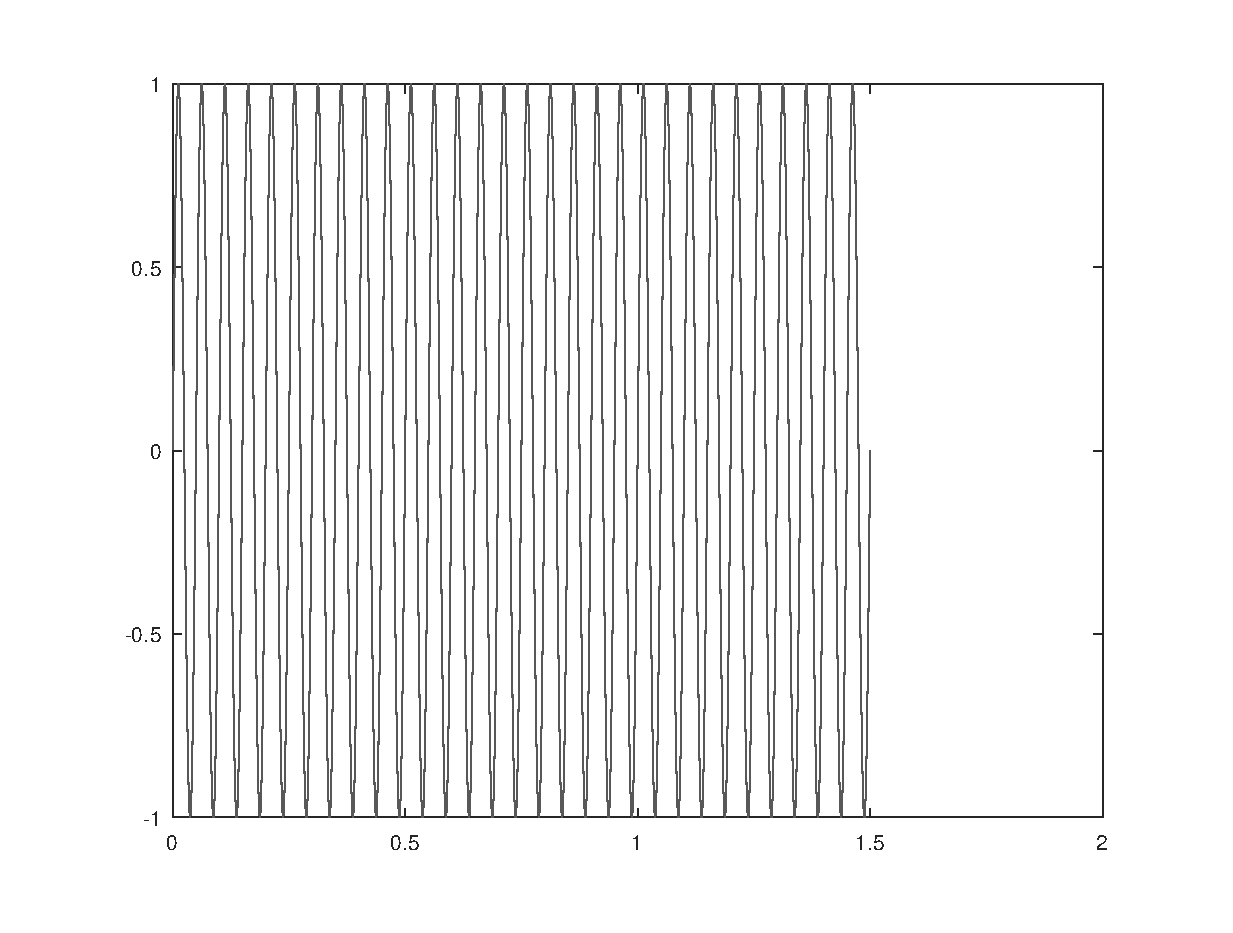
\includegraphics[width=8cm]{figures/modulaciok_workshop_szinusz.eps}
\caption{20 Hz-es szinusz függvény ábrázolása időtartományban}
\label{fig:szinusz}
\end{center}
\end{figure}

A 20 Hz-es jelet könnyen ábrázoltuk, de a hallható tartomány magasabb frekvencián van. Változtassuk a jel frekvenciáját 440 Hz-re (zenei A hang), és játsszuk ki a számítógép hangkártyáján a jelet:

\lstinline{soundsc(y, Fs); % Hang lejatszasa Fs mintaveteli frekvenciaval } 


Itt már több információt kapnánk a jelről, ha frekvenciatartományban, vízesés diagramon ábrázolnánk a jelet. A HA5KFU Octave gyakorlathoz csomagolt \textit{wf(y, Fs)} függvénnyel ezt a rádiózásban megszokott formában rajzolhatjuk ki. 

\lstinline{wf(y, Fs); % Vizeses diagram kirajzolasa }  

\begin{figure}[H]
\begin{center}
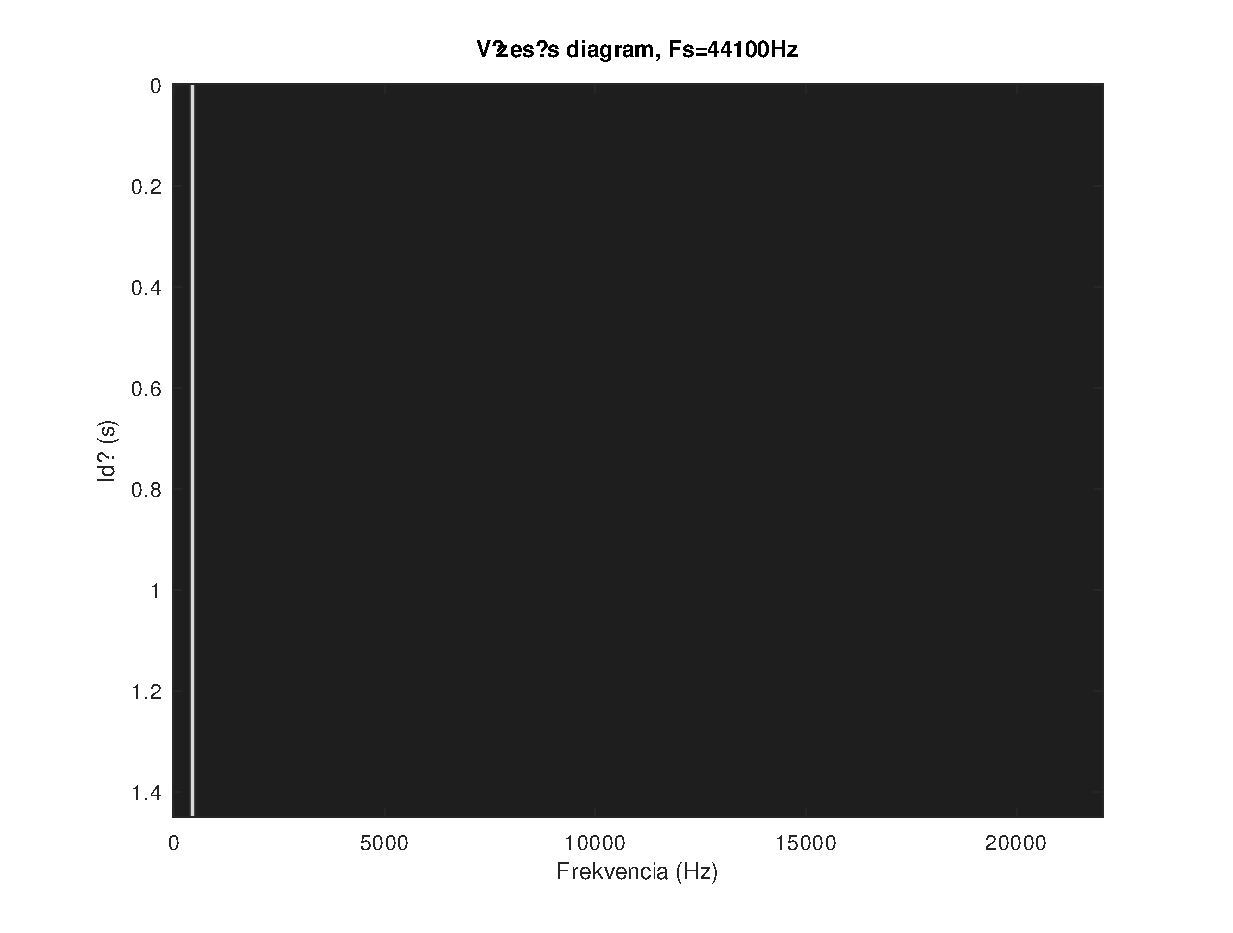
\includegraphics[width=8cm]{figures/modulaciok_workshop_waterfall.eps}
\caption{440 Hz-es szinusz függvény ábrázolása frekvenciatartományban}
\label{fig:waterfall}
\end{center}
\end{figure}

A vízesés diagram 0-tól a mintavételi frekvencia feléig ábrázolja a frekvenciakomponenseket, az ábrán láthatjuk a konstans szinusz jel képét 440 Hz-nél. Próbálkozzunk meg a jel manipulálásával, hallgassuk meg, ábrázoljuk frekvenciatartományban!\\
\lstinline{y = ( 1 - ( 1 / l ) * t ) .* sin( t * f * 2 * pi ); % Fokozatosan halkulo jel } \\
\lstinline{y = sin( t .* ( f * t ) * 2 * pi ); % Valtozo frekvenciaju szinusz } \\
\lstinline{y = sin( t * f * 2 * pi ) + sin( t * 1.5*f * 2 * pi ) ; % Tobb szinusz osszege }
\\
Megpróbálhatunk fehér zajt generálni, vagy hangfilet betölteni is. \\
\lstinline{y = rand( N, 1 ) ; % N elemu zaj}  \\
\lstinline{[y,Fs] = audioread( 'akkord.wav' ); N = length( y ); l=N/Fs; % WAV file beolvasasa}


\clearpage

\subsection{Keverés}


\begin{figure}[H]
\label{fig:keverok}
\centering
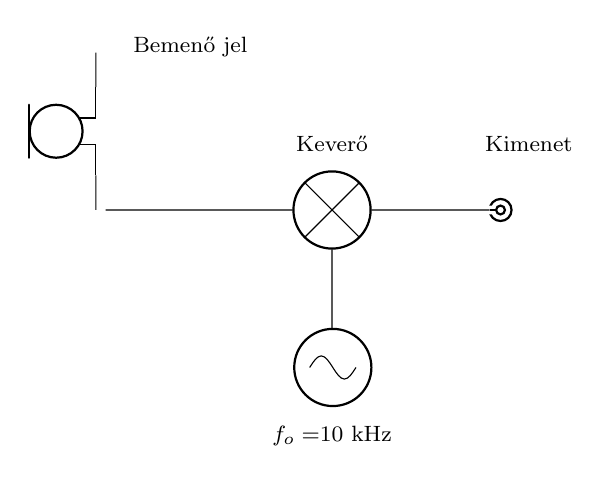
\begin{tikzpicture}

	\draw
	(5,0)node[bnc, xscale=-1] (bnc){}	
	(0,0) to[mic, name=M] ++(0,2)
	(1.2,1.7) node[label={[font=\footnotesize]above:Bemenő jel}] {}

	(3,-2.5) node[label={[font=\footnotesize]below:$f_o=$10 kHz}] {}
	
	(3,0.5) node[label={[font=\footnotesize]above:Keverő}] {}
	(5.5,0.5) node[label={[font=\footnotesize]above:Kimenet}] {}
	
	(0,0)[mic]node(mic){}
	(3,0)[mixer] node(mix){}	
	
	(3.5,-2)[oscillator] node(osc){}	
	(mic) to [short] ++(2.5,0) 
	(3,-1.5) to [short] (3,-0.5)
	(3.5,0) to [short] (5,0)
	
	;
    \end{tikzpicture}
\caption{
A keverő blokkvázlata} 
\end{figure}

Amikor egy jelet egy szinusz oszcillátor jelével keverünk (szorzunk), a jel megjelenik a frekvenciatartományban a két frekvencia összegeként és különbségeként. Ha pl a két jel egy $\omega_1$ frekvenciájú koszinusz vivő, és egy $\omega_2$ frekvenciájú koszinusz moduláló jel, a modulációs tétel alapján:

\begin{equation}
\cos(\omega_1t) \cdot \cos(\omega_2t) = \frac{1}{2}\cos(\omega_1t+\omega_2t) +  \frac{1}{2}\cos(\omega_1t - \omega_2t)
\end{equation}

Nézzük meg a gyakorlatban, próbáljuk meg az \textit{akkord.wav} hangfilet keverni, például egy 10 kHz-es szinusz jellel!


\begin{lstlisting}[frame=single,language=matlab,caption=Keverés]
[a,Fs] = audioread('akkord.wav'); N=length(a);
f = 10000; % 10 kHz-es lesz a vivo jel
t = ( 1:N )' ./ Fs;
b = sin( t * f * 2 * pi );

m = 0.75; % modulacios index
dc_offset = (1 + 1-m) * max(a);
a_dc = a + dc_offset; % dc eltolas
y = a_dc .* b; % a .* b


wf(y, Fs);
\end{lstlisting}

Vajon hogyan kapjuk vissza a kevert jelből az eredeti információt?

\clearpage

\subsection{IQ moduláció}



\begin{figure}[H]
\label{fig:iq}
\centering
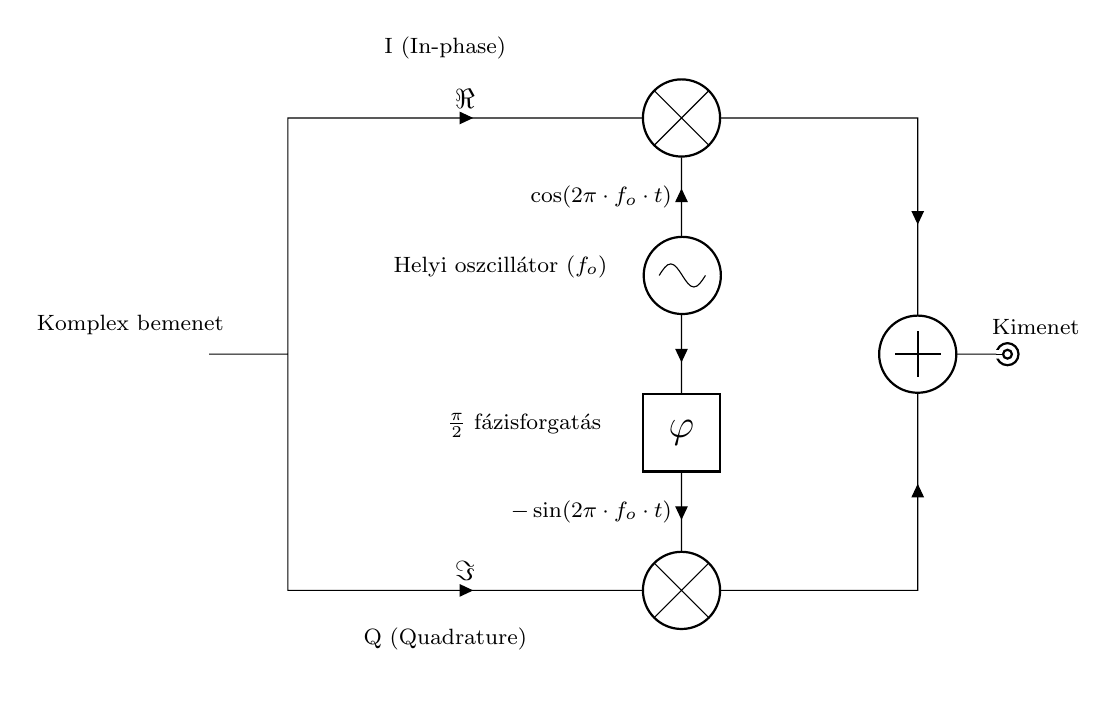
\begin{tikzpicture}

	\draw
	(10,-3)node[bnc, xscale=-1] (bnc){}	
	(-1,-3) node[label={[font=\footnotesize]above:Komplex bemenet}] {}
	
	(3.7,-1.5) node[label={[font=\footnotesize]below:Helyi oszcillátor ($f_o$)}] {}
	(4,-3.5) node[label={[font=\footnotesize]below:$\frac{\pi}{2}$ fázisforgatás}] {}
	(3,0.5) node[label={[font=\footnotesize]above:I (In-phase)}] {}
	(3,-7) node[label={[font=\footnotesize]above:Q (Quadrature)}] {}
	(10.5,-3) node[label={[font=\footnotesize]above:Kimenet}] {}
	
	(0, -3) to [short] ++(1,0) 
	(1,-3) to [short] ++(0,3) to [short, i=$\Re$] ++(4.5,0) 
	(1,-3) to [short] ++(0,-3) to [short, i=$\Im$] ++(4.5,0) 	
	
	(6,-1.5) to [short, i=\footnotesize $\cos(2\pi \cdot f_o \cdot t)$] (6,-0.5)
	
	(6,-2.5) to [short, i=\phantom{}] (6,-3.5)
	
	(6,-4.5) to [short, i>_=\footnotesize $-\sin(2\pi \cdot f_o \cdot t)$] (6,-5.5)
	
	(6.5,0) to [short] ++(2.5,0) to [short, i=\phantom{}] ++(0,-2.5) 
	(6.5,-6) to [short] ++(2.5,0) to [short, i=\phantom{}] ++(0,2.5) 
	(9.5,-3) to [short] ++(0.5,0)
	(6,0)[mixer] node(mixa){}	
	(6,-6)[mixer] node(mixb){}	
	

	(6.5,-2)[oscillator] node(osc){}	
	(6,-4)[phaseshiftershape] node(phas){}	
	
	(9,-3)[adder] node(add){}	
	
	;
    \end{tikzpicture}
\caption{
Az IQ modulátor blokkvázlata} 
\end{figure}

Az IQ modulátornál egy komplex jellel moduláljuk a vivő frekvenciát. Ezzel a módszerrel az alapsávi jelet egy komplex fazorként ábrázolhatjuk, és ez nagyban megkönnyíti a modulációs műveletek elvégzését.

\subsubsection{Fázismoduláció}

Készítsünk fázismodulátort IQ moduláció segítségével! Legyen az átvinni kívánt (moduláló) jel $x(t)$ (ügyelve arra, hogy $\vert x(t) \vert<1$)! Ekkor a $c(t)$ komplex vektor hossza $\vert c(t) \vert = 1$, fázisa pedig a modulált jel pillanatnyi értéke ($\arg\left(c(t)\right)=x(t) \cdot \pi$). Így a jel 1 értéke a $\pi$ fázishoz kerül. A $c(t)$ jelet az Euler alakkal könnyen előállíthatjuk: $c(t)=e^{j \cdot \pi \cdot x(t)}$.

\begin{figure}[H]
\begin{center}
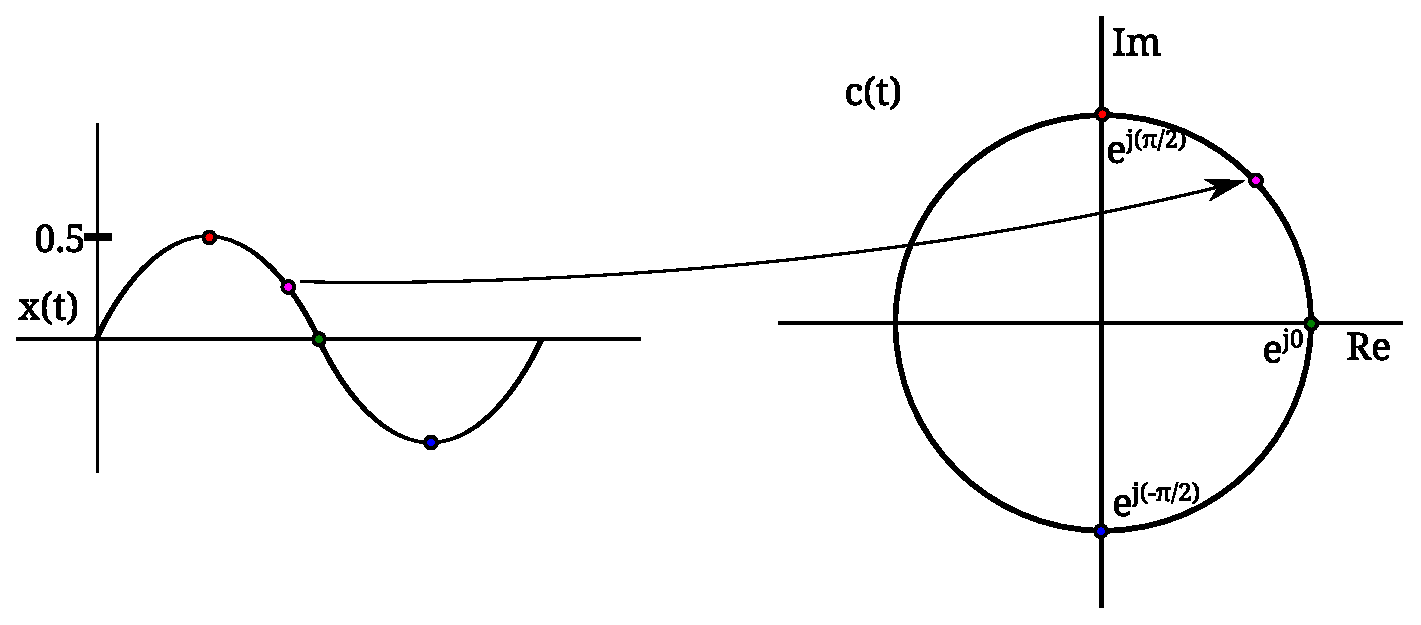
\includegraphics[width=13cm]{figures/modulaciok_workshop_pm.eps}
\caption{Fázisok előállítása a moduláló jelből}
\label{fig:pm}
\end{center}
\end{figure}

Az IQ keveréshez ennek a komplex jelnek a valós részét az in-phase $\cos(2\pi \cdot f_o \cdot t)$, a képzetes részét a quadrature $-\sin(2\pi \cdot f_o \cdot t)$ oszcillátor jellel moduláljuk (szorozzuk), majd összeadjuk. Kész is a modulált jel!

\begin{figure}[H]
\begin{center}
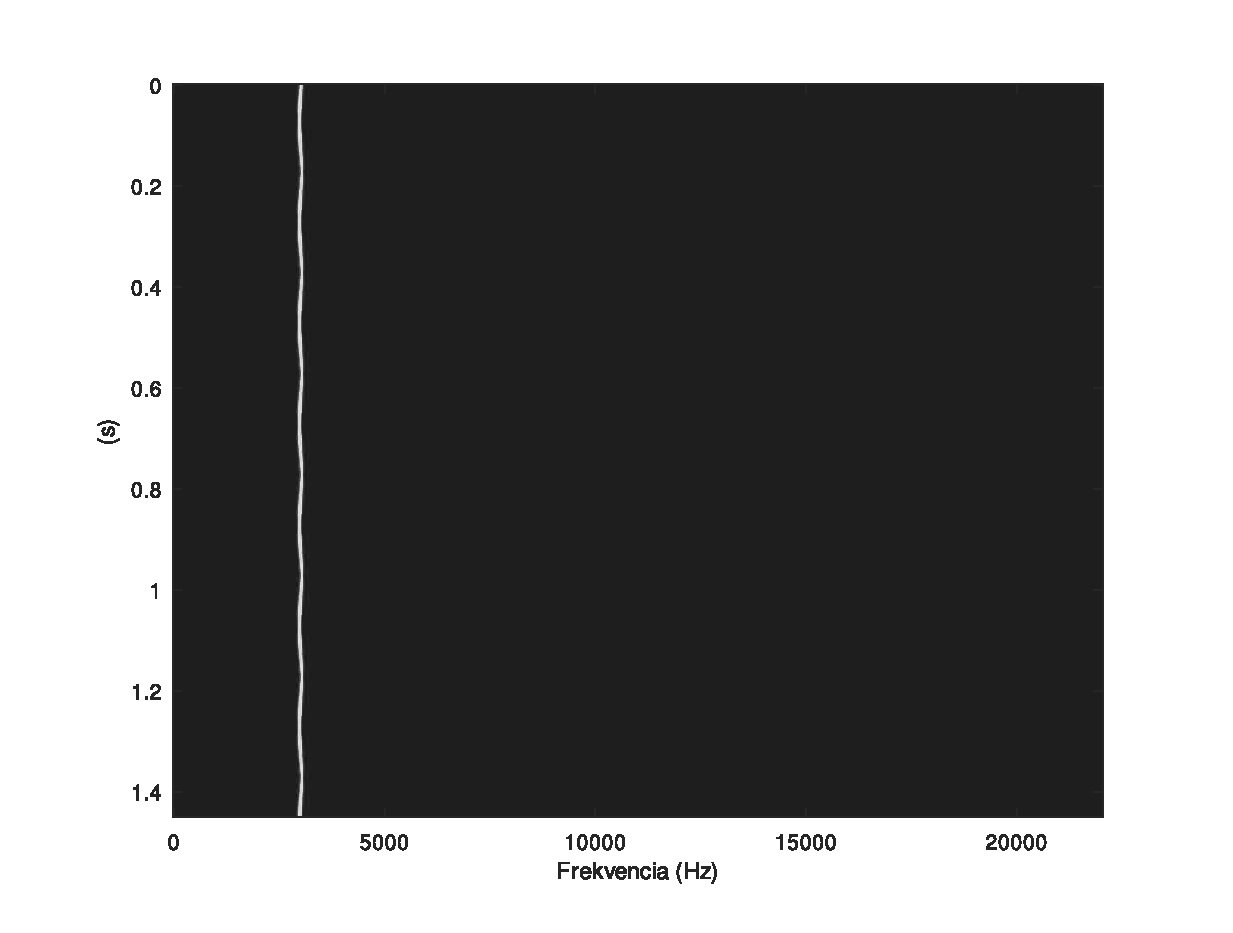
\includegraphics[width=8cm]{figures/modulaciok_workshop_phase.eps}
\caption{Az előállított fázismodulált jel}
\label{fig:phase}
\end{center}
\end{figure}
\clearpage
\begin{lstlisting}[frame=single,language=matlab,caption=Fázismoduláció IQ modulátorral]
Fs = 44100; % mintaveteli freki
l = 1.5; % minta hossza masodpercben
N = l * Fs; % mintak szama
t = ( 1:N )' ./ Fs; % Ido oszlopvektora

f = 5; % eredeti jel frek
x =  sin( t * f * pi ) .* 0.5; % ez lesz az atvinni kivant jel (1/2 amplitudo)

c = ones(N,1); % N meretu vektor letrehozasa es feltoltese 1-essel
for i=1:N
  c(i) = exp( j * 2 * pi * x(i) ); % fazismodulalt jel letrehozasa
end

fo = 3000; % oszcillator frek
oi =  cos( t * fo * 2 * pi ); % in-phase oszcillator
oq = -sin( t * fo * 2 * pi ); % quadrature oszcillator

y = oq .* imag(c) + oi .* real(c); % IQ keveres

figure(1);
plot(t, y);
figure(2);
wf(y, Fs);
\end{lstlisting}

Ez alapján készítsünk el egy FM modulátort! Nagyon hasonlít az előzőhöz, csak itt a komplex vektor forgásának frekvenciája változik.

\subsection{Újramintavételezés}

Próbáljuk ki hangfileokkal! Ügyeljünk arra, hogy a FM sávszélessége nagy lesz, ezért nagyobb helyre lesz szükségünk a frekvenciatartományban. Ha megváltoztatjuk a mintavételi frekvenciát és a hangot újramintavételezzük ez alapján, ki tudjuk terjeszteni a frekvenciatartomány méretét. \\
Vigyázzunk, hogy $n$-szeres mintavételi frekvenciánál a minták száma is $n$-szeresére változik, és ez nagyon megnövelheti a számítási időt. \\
Az újramintavételezés a \textit{resample(x, p, q)} függvénnyel tehető meg, ami $\frac{p}{q}$-szorosára változtatja a mintavételi frekvenciát (ehhez be kell tölteni a signal csomagot). Ne felejtsük a $F_s$ változót is beállítani!
\begin{lstlisting}[frame=single,language=matlab,caption=Újramintavételezés]
[x,Fs] = audioread('voice.wav');
% Ujramintavetelezes -> nagyobb frekitartomany
Fs = Fs * 4;
x = resample(x, 4, 1);
N = length( x ); l = N / Fs;
\end{lstlisting}

\end{document}



